\documentclass[male,czech]{kithesis}

\usepackage{graphics}
\usepackage{array}

% zde nastavte základní informace o bakalářské práci
\newcommand{\AUTOR}{Oleg Musijenko}
\newcommand{\TITULcz}{Tacit programming - návrh doménově specifického jazyka a implementace jeho interpretu} % titul v českém jazyce
\newcommand{\TITULen}{Tacit programming - design of a domain specific language and implementation of it's interpreter} % titul v anglickém jazyce
\newcommand{\KLICOVASLOVAcz}{bakalářská práce, odborný text, programování} % klíčová slova v českém jazyce
\newcommand{\KLICOVASLOVAen}{bachelor thesis} % klíčová slova v anglickém jazyce
\newcommand{\VEDOUCI}{Mgr. Jiří Fišer, Ph.D.}    

\newcommand{\PROGRAM}{Aplikovaná informatika}    
\newcommand{\OBOR}{Informační systémy}    
% nastavení fontů (liší se podle TeXovského stroje)
\iftutex
\usepackage{fontspec}
\setmainfont{Libertinus Serif} % použito je opensource písmo Libertinus, lze použít jakékoliv jiné rozumné
\setsansfont{Libertinus Sans}
\setmonofont[Scale = MatchLowercase]{Libertinus Mono}
%\setmainfont{APL385}
\newfontfamily\apl{APL385}
\usepackage{unicode-math}  
% písmo pro matematiku, vhodná písma viz  	např. https://developer.mozilla.org/en-US/docs/Mozilla/MathML_Project/Fonts
\setmathfont{Libertinus Math}
\else
\usepackage[utf8]{inputenc}
\usepackage[T1]{fontenc}
\usepackage{libertinus}

\usepackage{amsmath,amssymb}
\usepackage{libertinust1math}
\usepackage{graphicx}
\usepackage[font=small, labelfont=bf]{caption}
\fi

\usepackage[
  backend=biber,
  style=iso-authoryear,
  ]{biblatex}
\usepackage{minted}
\usepackage{listings}
\usepackage[dvipsnames]{xcolor}

% \newcommand\mkbibcolor[2]{\textcolor{#1}{\hypersetup{citecolor=#1}#2}}
% \DeclareCiteCommand{\cite}[\mkbibcolor{red}]
%   {\usebibmacro{prenote}}%
%   {\usebibmacro{citeindex}%
%    \usebibmacro{cite}}
%   {\multicitedelim}
%   {\usebibmacro{postnote}}

\definecolor{CodeBackGround}{cmyk}{0.0,0.0,0,0.05}  % light gray
\definecolor{CodeComment}{rgb}{0,0.50,0.00}         % dark green {0,0.45,0.08}

\addbibresource{bibliografie.bib}
% vylepšení vzhledu
\usepackage{microtype}
%\sloppy %odpoznámkujte pokud vám často přetékají řádky
\renewcommand{\arraystretch}{1.23} % vertikální roztažení tabulek o 23%


% Source from: https://github.com/bakerjd99/jacks/blob/master/latex/apl-lstlisting.tex
\lstdefinelanguage{apl}
{
extendedchars=true,
morekeywords={},
otherkeywords={:if,:else,:for,:in,:while,:until
,:andif,:orif,:repeat,:select,:case
,:go,:return,:try,:catch,:catchif,:catchall
,:endfor,:endwhile,:endselect,:endif,:endrepeat,:endselect},
keywordstyle=\bfseries\color{red},
sensitive=True,
morecomment=[l]{⍝}
}
\setmonofont{APL385}

\lstset{%
  basicstyle=\ttfamily\small,  
  keywordstyle=\bfseries\normalsize,  % can color key words        
  identifierstyle=,                             
  commentstyle=\slshape\color{CodeComment}, % no slanted shape in APL385    
  stringstyle=\ttfamily,                        
  showstringspaces=false,                      
  framesep=1pt,                                
  framerule=0.8pt,                              
  breaklines=true,      % break long code lines                        
  breakindent=0pt                             
}

\makeatletter
\lst@InputCatcodes
\def\lst@DefEC{%
 \lst@CCECUse \lst@ProcessLetter
  ^^80^^81^^82^^83^^84^^85^^86^^87^^88^^89^^8a^^8b^^8c^^8d^^8e^^8f%
  ^^90^^91^^92^^93^^94^^95^^96^^97^^98^^99^^9a^^9b^^9c^^9d^^9e^^9f%
  ^^a0^^a1^^a2^^a3^^a4^^a5^^a6^^a7^^a8^^a9^^aa^^ab^^ac^^ad^^ae^^af%
  ^^b0^^b1^^b2^^b3^^b4^^b5^^b6^^b7^^b8^^b9^^ba^^bb^^bc^^bd^^be^^bf%
  ^^c0^^c1^^c2^^c3^^c4^^c5^^c6^^c7^^c8^^c9^^ca^^cb^^cc^^cd^^ce^^cf%
  ^^d0^^d1^^d2^^d3^^d4^^d5^^d6^^d7^^d8^^d9^^da^^db^^dc^^dd^^de^^df%
  ^^e0^^e1^^e2^^e3^^e4^^e5^^e6^^e7^^e8^^e9^^ea^^eb^^ec^^ed^^ee^^ef%
  ^^f0^^f1^^f2^^f3^^f4^^f5^^f6^^f7^^f8^^f9^^fa^^fb^^fc^^fd^^fe^^ff%
  ^^^^20ac^^^^0153^^^^0152%
  ^^^^20a7^^^^2190^^^^2191^^^^2192^^^^2193^^^^2206^^^^2207^^^^220a%
  ^^^^2218^^^^2228^^^^2229^^^^222a^^^^2235^^^^223c^^^^2260^^^^2261%
  ^^^^2262^^^^2264^^^^2265^^^^2282^^^^2283^^^^2296^^^^22a2^^^^22a3%
  ^^^^22a4^^^^22a5^^^^22c4^^^^2308^^^^230a^^^^2336^^^^2337^^^^2339%
  ^^^^233b^^^^233d^^^^233f^^^^2340^^^^2342^^^^2347^^^^2348^^^^2349%
  ^^^^234b^^^^234e^^^^2350^^^^2352^^^^2355^^^^2357^^^^2359^^^^235d%
  ^^^^235e^^^^235f^^^^2361^^^^2362^^^^2363^^^^2364^^^^2365^^^^2368%
  ^^^^236a^^^^236b^^^^236c^^^^2371^^^^2372^^^^2373^^^^2374^^^^2375%
  ^^^^2377^^^^2378^^^^237a^^^^2395^^^^25af^^^^25ca^^^^25cb%  
  ^^00}
\lst@RestoreCatcodes
\makeatother

% \lstset{ %
%   language=Haskell,                % hlavní programovací jazyk, seznam podporovaných viz https://en.wikibooks.org/wiki/LaTeX/Source_Code_Listings
%   basicstyle=\ttfamily,    
%   showspaces=false,                % show spaces adding particular underscores
%   showstringspaces=true,           % underline spaces within strings
%   showtabs=false,                  % show tabs within strings adding particular underscores
%   frame=single,                    % adds a frame around the code
%   tabsize=3,                       % sets default tabsize to 3 spaces
%   breaklines=true,                 % sets automatic line breaking
%   breakatwhitespace=false,         % sets if automatic breaks should only happen at whitespace
%   keywordstyle=\bfseries,          % keyword style
%   commentstyle=\rmfamily,          % comment style
%   stringstyle=\itshape,            % string literal style
% }

% nastavení hypertextových odkazů a PDF metainformací
\usepackage{url} % přidává příkaz url pro sazbu url
\usepackage[unicode=true,colorlinks=true,
            citecolor=blue, linkcolor=blue,
            urlcolor=blue,
            pdftitle={\TITULcz},pdfauthor={\AUTOR},
            pdfkeywords={\KLICOVASLOVAcz}]{hyperref}

\usepackage[skip=10pt plus1pt]{parskip}
\newcommand{\haskellInline}[1]{\colorbox{gray!10}{\mintinline{haskell}{#1}}}
\newcommand{\aplInline}[1]{\colorbox{gray!10}{{\apl{#1}}}}

\pagestyle{fancy} % aktivování stylu záhlaví a zápatí z kithesis

%---------------------------------------------------------

\begin{document}
\thispagestyle{empty}
\begin{center}
{\Huge Univerzita Jana Evangelisty Purkyně \\
v~Ústí nad Labem}
\\[16pt]
{\huge Přírodovědecká fakulta}

\vspace{2cm}
\resizebox{8cm}{!}{
\includegraphics{LOGO_PRF_CZ_RGB_standard.jpg}}

\vspace{2cm}
{
\huge
\TITULcz\par

\vspace{0.5em}
\LARGE\scshape bakalářská práce
}
\end{center} 
 
\vfill
{
\large
\begin{tabular}{>{\bfseries}rl}
    Vypracoval: 	& \AUTOR\\
    Vedoucí práce: 	& \VEDOUCI\\
&\\
Studijní program:       & \PROGRAM\\
Studijní obor:          & \OBOR\\
\end{tabular} 
}
\vspace{1.5cm}
\begin{center}
\Large\scshape   Ústí nad Labem \the\year
\end{center}

\cleardoublepage
\thispagestyle{empty}

\textbf{\textsf{Cíl bakalářské práce}}

Cílem bakalářské práce je ukázat výhody a nevýhody tacit přístupu k programování. Výstupem práce bude návrh vlastního doménově specifického jazyka (DSL), který
bude využívat tacit programming, a navazující pilotní implementace jeho interpretu.
Návrh jazyka by se měl soustředit na následující body:\\
• přehledná syntaxe,\\
• možnosti použití vysokoúrovňových nástrojů pro překlad a podporu běhu programu (např. LLVM v Haskellu) včetně parsování jazyka (např. Parsec v Haskellu),\\
• efektivita při vykonávaní,\\
• případná podpora paralelních výpočtů

\cleardoublepage
\thispagestyle{empty}

\textbf{Prohlášení}

Prohlašuji, že jsem tuto bakalářskou práci vypracoval\ifthenelse{\boolean{feminum}}{a}{} samostatně a použil\ifthenelse{\boolean{feminum}}{a}{}
jen pramenů, které cituji a uvádím v přiloženém seznamu literatury.

\vspace{1em}
Byl\ifthenelse{\boolean{feminum}}{a}{} jsem seznámen\ifthenelse{\boolean{feminum}}{a}{} s tím, že se na moji práci vztahují práva a povinnosti vyplývající ze zákona č. 121/2000 Sb., ve znění zákona č. 81/2005 Sb., autorský zákon, zejména se skutečností, že Univerzita Jana Evangelisty Purkyně v Ústí nad Labem má právo na uzavření licenční smlouvy o užití této práce jako školního díla podle § 60 odst. 1 autorského zákona,s tím, že pokud dojde k užití této práce mnou nebo bude poskytnuta licence o užití jinému
subjektu, je Univerzita Jana Evangelisty Purkyně v Ústí nad Labem oprávněna ode mne požadovat přiměřený příspěvek na úhradu nákladů, které na vytvoření díla vynaložila, a to podle okolností až do jejich skutečné výše.

\vspace{1em}
V Ústí nad Labem dne \today \hspace{0.3\textwidth} Podpis:


\clearpage
\thispagestyle{empty}
~\vfill

\begin{flushright}
  Děkuji vedoucímu práce Mgr. Jiřímu Fišerovi, Ph.D.\\ za neocenitelné rady a pomoc při tvorbě bakalářské práce.

  Též chci poděkovat své ženě, Anetě Musijenko, \\ za neustálou podporu během psaní práce.
\end{flushright}

\cleardoublepage
\thispagestyle{empty}

\textbf{\textsf{Abstrakt}}

\textsc{\TITULcz}

Cílem této bakalářské práce je vytvoření doménově specifického jazyka se zaměřením na konkurentní výpočty, 
který usnadní přehled business logiky a zlepší vývojářské prostředí (developer experience) se zaměřením na \textit{tacit} - "beztečkové" paradigma.
V práci se nachází ukázky, 
jak tacit programming vypadá a 
jsou zde vyzdvyženy argumenty proč psát programy tacitně.
Ukázky v této práci potvrzují, 
že jazyky které nebyly primárně navržené jako "beztečkové" 
umožňují v tomto stylu psát.
Nadále se zde nachází obecné vysvětlení, 
jak parsovat jazyk pomocí knihovny Parsec a
jak užít výsledek parsování do metaprogramming mechanismu "Template Haskell".
Byly vytvořeny tři ukázky, 
které validují užití vytvořeného DSL a
nachází se diskuze o možných budoucích vylepšení.

% Abstrakt shrnuje základní motivaci práce (kontext), hlavní cíl a následně jednotlivé
% autorské kroky k~jeho splnění (co bylo uděláno od úvodních rešerší, přes návrh, implementaci k případnému nasazení. Minimální rozsah je 800 znaků (maximální půl strany).

\textbf{\textsf{Klíčová slova}}

Haskell, Doménově specifický jazyk, Beztečkové programování, Konkurence, Parser, Template Haskell, Metaprogramming

% seznam klíčových slov (obecných termínů vystihujících téma práce) v počtu dva až deset 

\vspace{1em}
\hrulefill
\vspace{1em}

\textbf{\textsf{Abstract}}

\textsc{\TITULen}


The aim of this bachelor thesis is to create a 
domain-specific language focusing on concurrent computations, 
which will facilitate understanding of business logic and 
enhance developer experience by targeting the tacit paradigm. 
The thesis contains examples illustrating what 
tacit programming looks like and 
highlights arguments for writing programs tacitly. 
The examples in this work confirm that 
languages not primarily designed as "tacit" allow writing in this style.
Furthermore, 
there is a general explanation 
of how to parse the language using the Parsec library and 
how to utilize the parsing result in 
the metaprogramming mechanism "Template Haskell". 
Three examples have been created to validate the use of the created DSL,
and there is a discussion about possible future enhancements.

\textbf{\textsf{Key words}}

Haskell, Domain Specific Language, Tacit programming, Concurrency, Parser, Template Haskell, Metaprogramming

{
  \hypersetup{linkcolor=black}
  \tableofcontents
}

\addchap{Úvod}

V současnosti se vyrábí procesory s co největším počtem jader, 
a tím pádem i vláken, 
i přesto,
že je velmi náročné pro jednu aplikaci tyto další vlákna využít.
Objevují se zde často potíže se stavem programu,
kde se musí daný stav šířit napříč různými vlákny.
Proto cílem této bakalářské práce bylo vytvořit DSL, 
který má pomoci s pochopením přenosu dat mezi různými vlákny
a vyřešit problémy spjaté s přenosem,
což má za následek snažší přístup k dalším počítačovým zdrojům.
Pro implementaci DSL byl využit programovací jazyk Haskell a 
v práci se nachází odůvodnění,
proč byl tento jazyk zvolen. 

V první kapitole se nachází vysvětlivka programovacích paradigmat a 
jak vypadá tacitní syntaxe, 
protože navržené DSL využívá tuto syntaxi. 
V druhé kapitole se nachází využití různých DSL v závisloti na kontextu projektu.
Ve třetí kapitole se může čtenář dočíst, 
jak došlo k navržení DSL a 
v následující kapitole jak došlo k implementaci v jazyce Haskell.
V předposlední kapitole se nachází tři praktické ukázky, 
jak lze takové DSL využít.
V poslední kapitole jsou vytknuty nedostatky implementace a
kde by mohlo dojít k vylepšení. 

Před studováním této bakalářské práce se doporučuje znát základy funkcionálního programování a
to konkrétně Haskellu.
Nachází se zde příklady,
které se srovnávají s jazykem C nebo JavaScriptem.
Návrh je vytvořen v Haskellu pomocí knihoven jako
jsou Parsec a MTL (Monad Transformer Library).

\chapter{Programovací paradigma a tacit programming}

Programovací paradigma je způsob myšlení a přístupu k návrhu, 
strukturování a 
implementaci počítačových programů. 
Definuje sadu pravidel, postupů, technik a konceptů, 
které určují způsob,
jakým se programy píší a organizují. 
Paradigma poskytuje rámec pro definici a 
řešení problémů v programování.

Některé z nejznámějších programovacích paradigmat zahrnují 
procedurální, objektově orientované a funkcionální.
Na různá paradigmata má zároveň vliv způsob 
správy paměti.

\section{Vysvětlení paradigmat}

Procedurální paradigma se zaměřuje na sekvenci instrukcí, 
které jsou vykonávány postupně
v závislosti na architektuře procesoru.
Program je rozdělen na procedury a funkce, 
které provádějí určité operace. (\cite{Martin2018}, s. 48-49)

Objektově orientované paradigma klade důraz na objekty a
jejich interakce. 
Program je strukturován kolem tříd, 
které obsahují data (atributy) a 
metody (funkce), 
které s těmito daty pracují. (\cite{Martin2018}, s. 49)

Funckionálního paradigma je deklarativní způsob programování, 
kde funkce jsou považovány za základní stavební bloky programu. 
Funkcionální jazyky mají za cíl minimalizovat vedlejší efekty.
To přispívá ke stabilitě, zjednodušení problematiky domény a 
eliminaci některých typů chyb. (\cite{Martin2018}, s. 49)

V různých funkcionálních jazycích je povolena různá míra mutace dat.
Například jazyk F\# umožňuje mutaci dat kdekoli v programu, 
což je částečně záměrem, 
aby uživatelé jiných programovací jazyků měli snažší přenos svých vědomostí do 
nového prostředí.
Na druhou stranu, 
v jazyce Haskell jsou mutace omezeny v IO monádě a 
data musí být uloženy 
ve specifických typech jako IORef, STRef nebo MVar (\cite{Jones2010}). 
Takto Haskell pomáhá udržet jasnou separaci mezi čistým funkcionalním kódem a kódem, 
který se zabývá měnícím se stavem nebo interakcí s okolím.

Je důležité si uvědomit, 
že míra povolené mutace dat se může lišit mezi jednotlivými funkcionálními jazyky a 
je závislá na jejich návrhu a filozofii. 
Každý jazyk si volí kompromis mezi funkcionalitou a 
striktností v oblasti mutace, 
aby splňoval požadavky svých uživatelů a cílů, 
které si klade.

\section{Vliv paradigmat na programovací jazyky}
Velmi málo jazyků implementuje paradigma stoprocentně. 
Když to udělají, 
jsou takzvaně \textit{čisté} (\cite{ProgrammingParadigms}). 
Je neuvěřitelně vzácné mít "čistě OOP" jazyk nebo 
"čistě funkcionální" jazyk. 
Haskell který se považuje za \textit{čistě} funkcionální jazyk,
tak podporuje \textit{do} notaci díky němuž se dá psát kód imperativně
i když se jedná o syntaktické cukrátko \textit{monad bind} operátoru.
Dalším příkladem je že velmi málo jazyků implementuje OOP, 
jak si jej Alan Kay představoval (\cite{ProgrammingParadigms}).
Mnoho jazyků usnadňuje programování v jednom nebo více paradigmat. 
V jazyce Scala můžete snadno provádět imperativní, 
objektově orientované a funkcionální programování. 
Pokud je jazyk úmyslně navržen tak, 
aby umožňoval programování v mnoha paradigmatech současně, 
nazýváme ho jazykem s více paradigmaty. 
Pokud jazyk neúmyslně podporuje více paradigmat, 
neexistuje pro to zvláštní slovo (\cite{ProgrammingParadigms}).

\section{Tacit programming}

Tacit programming je programovací styl, 
který klade důraz na kompozici funkcí, 
které manipulují argumenty a 
kde se tyto argumenty explicitně nespecifikují (\cite{Barros2005}).
Základní principy funkcionálního a tacit programování jsou v jazyce JavaScript,
jelikož se jedná o jeden z nejvíce populárních programovacích jazyků v roce 2023
a v základu má již funkcionální možnosti (\cite{StackSurvey}).
Detailnější principy jsou psány v Haskellu.

\textbf{Javascript}
\begin{minted}[bgcolor=CodeBackGround]{js}

  fetch("APIURL")
  .then(x => fancyFunction(x))
  .then(x => console.log(x))
  .catch(e => console.error(e))

\end{minted}

Zde se řetězí funkce zpětného volání ("Callbacks"). 
Tento postup je běžný u JavasSript programátorů,
ale bohužel má jednu malou nevýhodu.
Tvoří se zde zbytečná anonymní funkce ("arrow function nebo-li šipková") 
a pokud bychom prohlubovali čím dál víc zásobník volání,
mohou nám tyto anonymní funkce zabírat paměť a 
během debuggingu nám tento styl zápisu "znečišťuje" 
zásobník volání. 

\begin{minted}[bgcolor=CodeBackGround]{js}

  fetch("APIURL")
  .then(fancyFunction)
  .then(console.log)
  .catch(console.error)

\end{minted}

Přepsaná ukázka je logicky ekvivalentní k té předešlé. 
Zásadní rozdíl je ten, 
že se nemusí na paměťový zásobník ukládat kontext anonymní funkce 
a explicitně se nepředávají parametry funkce. 
Tudíž se jedná o \textit{tacit} zápis.

Následující úryvek ukazuje, 
jak funguje \textbf{currying} a proč souvisí s tacit programováním.

\textbf{Javascript}
\begin{minted}[bgcolor=CodeBackGround]{js}

const curry = (f) => a => b => f(a,b);
const sayHello = (a, b) = `Hello ${a} from ${b}`;
const applyToFunctionArray = 
    (input,...args) => args.map(a => a(input))
const partiallyAppliedData = ["A", "B", "C"].map(curry(sayHello)); 
// [(b) => "Hello A from ${b}", 
//  (b) => "Hello B from ${b}", 
//  (b) => "Hello C from ${b}"]
const partiallyAppliedData2 = ["A", "B", "C"]
                              .map(curry(sayHello)(1)); 
// ["Hello A from 1", 
//  "Hello B from 1", 
//  "Hello C from 1"]

\end{minted}
Curry funkce transfomuje existující funkci tak, 
že máme pro každý argument vlastní vracející funkci  (\cite{Currying}). 
Z funkce \textbf{f(a,b,c,d)} vzniká funkce \textbf{f(a)(b)(c)(d)}.
V čem je toto výhodné?
Například je zde uvedené pole, 
které se skládá z částečně aplikovaných funkcí. 
Takto může například programátor postupně naskládat výsledky opovědí ze serveru,
které je třeba závislé na uživatelském vstupu. 

Zajímavější část je u \textit{partiallyAppliedData2}. 
Curryovaná funkce vrací funkci, 
jež očekává vstupní parametr, 
aby byla vyhodnocena. 
Tento princip je důležitý
pro lenivé vyhodnocení, 
který využívá Haskell (\cite{HaskellCurrying}).

Může zde padnout argument, 
že ve zmíněném případě se curryování nachází pouze pro funkci,
která přijímá pouze dva argumenty. 
Zde je definice funkce, 
která převádí jakoukoliv funkci na curryovanou.

\textbf{Javascript}
\begin{minted}[bgcolor=CodeBackGround]{js}

const curry = (f) => (..args) => args.length >= f.length ? 
  f.apply(this, args) : (...args2) => 
    curry.apply(this, args.concat(args2));

\end{minted}

Nutné je zmínit, 
co \textbf{není} tacitní zápis. 
Řetězení metod nebo funkcí není jejich kompozicí!
Z definice tacit programmingu vyplývá,
že musí docházet ke kompozici funkcí bez specifikace parametrů a
ne řetězit funkce v závislosti na jejich typu nebo prototypu.

\textbf{C\#}
\begin{minted}[bgcolor=CodeBackGround]{csharp}

class MainClass 
{
  static void Main(string[] args)
  {
    string someString = Foo("Some argument");
  }

  static string Foo(string arg)
  {
      return new StringBuilder(argument)
      .Append("Hello")
      .Append(" ")
      .Append("World")
      .ToString();
  }
}

\end{minted}

Proč příklad se C\# není zapsán jako tacit? 
Funkce \textit{Append} vrací vlastní referenci na \textit{StringBuilder} a 
ne novou funkci. 
Též se zde pracuje s argumenty funkce, 
což je proti definici tacit programmingu.

\section{Využití Tacit programmingu v různých programovacích jazycích}

Tacit programming se dá pouze využít v jazycích,
které mají v sobě již zakomponované funkce jako hodnoty a
anonymní funkce nebo-li lambda výrazy.
Pokud jsou tyto podmínky splněné, 
tak lze obecně nadefinovat funkci pro kompozici i přesto,
že \textit{composed} funkce nebude syntakticky kompaktní.

Následující příklad sumace:

\textbf{Haskell}
\begin{minted}[bgcolor=CodeBackGround]{haskell}

sumCustom:: (Traversable t, Num a) => t a -> a
sumCustom = foldr (+) 0

\end{minted}

\textbf{C}
\begin{minted}[bgcolor=CodeBackGround]{c}

int sum(int* arr, size_t numOfElements)
{
    int acc = 0;
    
    for(int i = 0; i < numOfElements; i++)
    {
        acc += *(arr + i);
    }
    
    return acc;
}

\end{minted}
Z příkladu si lze povšimnout, 
že beztečkový styl zápisu je opravdu kompaktní. 
V Haskellu není třeba explicitně manipulovat s parametry funkcí.

Další příklad poukazuje Fibonacciho posloupnost.
\textbf{Haskell}
\begin{minted}[bgcolor=CodeBackGround]{haskell}

-- Haskell je lenivý jazyk a proto je možné vytvořit nekonečnou 
-- fibonnacciho posloupnost a z té si vzít jen potřebný počet čísel 
fibonacci:: Num a => Int -> [a]
fibonacci = (flip take) fibonacciInfinite
  where
    fibonacciInfinite:: Num a => [a]
    fibonacciInfinite = scanl (+) 0 (1:fibonacciInfinite)

\end{minted}

% \vfill
% \pagebreak

\textbf{C}
\begin{minted}[bgcolor=CodeBackGround]{c}

void fibonacci(uint* arr, size_t numOfElements)
{
    if(numOfElements > 0)
    {
      arr[0] = 0;
    }
    if(numOfElements > 1)
    {
      arr[1] = 1;
    }
    for(int i = 2; i < numOfElements; i++)
    {
      arr[i] = arr[i - 1] + arr[i - 2];
    }
}

\end{minted}

Z pohledu imperativního programátora implementace v C je zcela jasná. 
Funkce přijímá ukazatel na pole a modifikuje toto pole. 
Zatímco v Haskellu tato implementace může být matoucí. 
Funkce scanl je velice podobná funkci foldl, 
jen místo konečného vracení akumulátoru, 
tak vrací průběžně vypočtené hodnoty.

\section{Debugging}

Debugging je zásadní činností při vývoji softwaru, 
která umožňuje identifikovat, 
analyzovat a odstraňovat chyby ve zdrojovém kódu (\cite{WhatIsDebugging}). 
Proces debuggování je obzvláště důležitý v imperativních a objektově orientovaných jazycích, 
které často disponují vyspělými debugovacími nástroji.
V těchto jazycích je očekáváno sekvenční vykonávání instrukcí, 
což usnadňuje postupné sledování jejich provádění. 
Inspekce zásobníku volání představuje 
další přirozenou součást debuggingu v těchto jazycích.

V případě lenivého jazyka Haskell však debugging přináší značné obtíže. 
Haskell využívá mechanismu lenivého vyhodnocování, což znamená, 
že hodnoty jsou vypočteny až ve chvíli, kdy jsou skutečně potřeba (\cite{HaskellDebugging}).
Tato vlastnost komplikuje proces sledování výpočtu a identifikaci chyb. 
I přes existenci několika debuggovacích nástrojů pro Haskell může 
debugging pro zkušeného vývojáře představovat opravdovou výzvu. 
Zmatek může vznikat zejména při určování, 
kde a jak byla konkrétní proměnná získána, 
neboť její hodnota je vypočítána až v okamžiku, 
kdy je použita.

Naštěstí Haskell nabízí možnost využití REPL 
(Read - Eval - Print - Loop) prostředí, 
které umožňuje interaktivní evaluaci výrazů a postupné zkoumání jejich chování. 
REPL tak může sloužit jako užitečný nástroj pro rychlé testování 
a experimentování s funkcemi a výrazy \cite{HaskellGHCI}. 
Přítomnost REPL v Haskellu zčásti kompenzuje obtíže spojené 
s debuggingem a poskytuje prostředí pro analýzu a ladění kódu.

\section{Rešerše existujících implementací - APL}

Jazyk APL je jazyk orientovaný na pole nebo-li \textit{array oriented programming language} se 
syntaxí zaměřenou na tacit programming. V APL jsou všechny data reprezentovány jako pole 
a všechny pole jsou skládány ze skalárů a nad 
nimi jsou dělané matematické operace s poněkud netradiční syntaxí. Totiž každá 
předem jazykem definovaná funkce je přidělená ke speciálnímu UTF-8 chararakteru. 
Například funkce pro přirozený logaritmus je {\apl '⍟'} nebo zaokrouhlení nahoru či dolů 
jsou {\apl '⌈' '⌊'}.
Každá funkce se dá zapsat monadicky či dyadicky (\cite{WhyAPLIsWorthKnowing}).

Monadický zápis má argument operandu na pravé straně:
\aplInline{-5    ⍝ monadic}

Dyadický zápis má argumenty na obou stranách operandu:
\aplInline{10-7  ⍝ dyadic}

Jelikož všechny pole jsou tvořeny skaláry, tak operace "ignorují" strukturu pole a pracují přímo 
s obsahem pole.

\begin{lstlisting}[language=apl,extendedchars=true]
  ⍳6          ⍝ 6 integers starting from the origin.
0 1 2 3 4 5
  1+⍳6        ⍝ Add 1 to the 6 integers starting from the origin.
1 2 3 4 5 6
  2×⍳6        ⍝ Multiply by 2 the 6 integers starting from the origin.
0 2 4 6 8 10
\end{lstlisting} 

Pokud pole jsou u dyadického zápisu stejné délky, tak jsou hodnoty vypočteny jako jednotlivé 
skaláry.

\begin{lstlisting}[language=apl,extendedchars=true]
  100 0 1 × 2 3 4
200 0 4
\end{lstlisting}

Operátory jsou vyhodnocovány z prava do leva.

\begin{lstlisting}[language=apl,extendedchars=true]
  24 ÷ 12 6 - 4 2   ⍝ -> 24 ÷ 8 3
3 6
\end{lstlisting}

Zmíněné části kódu jsou vyjmuty z \cite{WhyAPLIsWorthKnowing}.

Booleany jsou reprezentovány jako 1 (True) a 0 (False). Zde je ukázka algoritmu, kde 
se sečte sekvence přirozených čísel (včetně nuly, ale při součtu nemá vliv), 
která jsou dělitelná buď třemi nebo pěti.

\begin{lstlisting}[language=apl,extendedchars=true]
  Euler1 ← {+/((0=3|⍵)∨(0=5|⍵))/⍵}

  Euler1 ⍳1000
234168
\end{lstlisting}

Funkce \aplInline{(0=3|⍵)∨(0=5|⍵) ⍝ '|' - modulo, 
'=' is equal operator} zjišťuje zda-li je číslo
dělitelné třemi nebo pěti a vrací 0 nebo 1. 
Operátor \aplInline{/} funguje jako replicate 
(pokud je spojené s dalším operátorem, 
tak funguje jako reduce). 
Jelikož je vyhodnocování z prava do leva, 
tak pokud argument funkce je 
například 7 a 12 tak: 

\aplInline{((0=3| 7 12)∨(0=10 | 7 12))/7 12 ⍝ Result: 12}.

Toto celé funguje jako filtrování, 
kombinací operátorů \aplInline{+/} se udělá suma výsledků.

Lze si ale povšimnout, 
že výše zmíněný příklad není zapsán v tacit stylu jelikož využívá argument \aplInline{⍵}.
Je možné napsat zmíněný příklad do tacit stylu, 
ale zároveň se zvyšuje komplexita porozumění.
\begin{lstlisting}[language=apl,extendedchars=true]
  Euler1 ← +/((0=3|⊢)∨(0=5|⊢))×⊢
\end{lstlisting}

Eulerova implementace a 
pochopení psaní tacit stylu v APL pomohl článek (\cite{CzechApl}).

\section{Kdy využít tacit zápis}

Tacit styl může být mocný a elegantní.
Zde je několik argumentů, 
proč by se měl tacit zápis využít:

\textbf{Kompaktnost a elegance:}
Tacitní zápis může často zredukovat kód na mnohem kratší a elegantnější formu, 
což může zvýšit čitelnost a snížit objem psaného kódu.

\textbf{Snížení chybovosti:}
Vzhledem k tomu, že tacitní zápis minimalizuje použití proměnných a stavu, 
může to snížit možnosti chyb spojených s nechtěnými efekty a nekonzistencemi v datech.

\textbf{Výkonové optimalizace:}
V některých případech může tacitní zápis vést k efektivnějšímu kódu, 
protože se snižuje zbytečná manipulace s proměnnými a daty.

\textbf{Snížení náročnosti na paměť:}
Tacitní zápis může minimalizovat požadavky na paměť tím, 
že eliminuje nutnost uchovávat mezivýsledky v proměnných.

\textbf{Zvyšuje jasnost:}
V některých případech může tacitní zápis zvýšit jasnost kódu tím, 
že se soustředí na to, co se děje (funkce a operace), 
a minimalizuje odvádějící pozornost od proměnných a argumentů.

\textbf{Kód s méně chybami:}
S minimálním množstvím stavových proměnných a 
nečekaných efektů může být kód napsaný v tacitním stylu méně náchylný k chybám.

\textbf{Přenositelnost:}
Tacitní zápis může být často snadněji přenositelný mezi různými jazyky nebo platformami, 
protože se soustředí na základní funkce a operace.

%%%%%%%%%%%%%%%%%%%%%%%%%%%%%%%%%%%%%%%%%

\section{Kdy se vyhnout tacit zápisu}

Bohužel tacit styl také může být obtížný pro programátory, 
zejména pokud nejsou na tento způsob programování zvyklí. 
Zde jsou argumenty proti tacit stylu:

\textbf{Složitost čtení a porozumění:} 
Tacitní styl může být velmi těžko čitelný a obtížný k pochopení, 
což může způsobit problémy v týmu a při údržbě kódu. 
Programátoři by měli být schopni snadno rozumět kódu,
který píšou, a kód napsaný v tacitním stylu může být matoucí.

\textbf{Náročná údržba:}
I když může být výrazně kratší, 
kód napsaný v tacitním stylu může být obtížný k úpravám a opravám chyb. 
Programátoři, kteří nejsou zvyklí na tento styl, 
budou mít problémy s debugováním a vylepšováním kódu.

\textbf{Nepodporované vývojářské prostředí:}
Některé programovací jazyky a prostředí nejsou vhodné pro zápis ve formě tacit, 
což může být dalším důvodem, proč by nemělo být programátorům vnucováno.

\textbf{Ztráta flexibility:}
Tacitní styl může omezit flexibilitu programátorů při psaní kódu.
Může být obtížnější provádět změny a úpravy v kódu, což může zpomalit vývoj.

\textbf{Vzdělávací nároky:}
Programátoři, kteří nejsou obeznámeni s tacitním stylem, 
budou muset investovat čas a úsilí do jeho pochopení a osvojení. 
To může zpomalit vývojový cyklus a zvyšovat náklady na vývoj.

\textbf{Nedostatek standardů:}
V různých programovacích jazycích mohou být různé konvence a 
standardy pro zápis ve formě tacit. To může způsobit nekonzistenci a zmatek mezi programátory.

\textbf{Kompromisy na úkor čitelnosti:}
Někdy se programátoři mohou pokoušet dosáhnout krátkého kódu na úkor čitelnosti a jasnosti. 
To může vést k nepřehledným a těžko udržovatelným programům.

%%%%%%%%%%%%%%%%%%%%%%%%%%%%%%%%%%%%%
\chapter{DSL - principy a využití}
DSL (Domain Specific Language) jsou jazyky, 
které se zaměřují na specifickou doménu problematiky.
Obecně DSL jazyky jsou mnohem jednodušší než jejich plnohodnotné protějšky. 
Výhodou je, 
že náročnost učení je mnohem nižší než u GPL (General Purpose Language). 
Zároveň při potřebě expertů na specializovaný obor, 
nepotřebují znát detaily implementace algoritmů, 
ale místo toho pokud budou mít přístup rovnou k DSL - výpočet šikmosti stěny budovy,
hodnota cukrů v krvi pacienta, 
tak mohou plnit svojí práci o mnohem efektivněji (\cite{DomainSpecificLanguages}).

\section{Web a enterprise}
Jedním z nejrozšířenejších DSL jazyků je ze světa webu a to \textbf{HTML a CSS}. 
HTML se zaměřuje na vytvoření rámce pro zobrazení textu,
zatímco CSS se zaměřuje na stylizaci webu pomocí DOM selectorů. 
Různé webové enginy renderují CSS jinak jelikož W3C standard neomezuje specifikaci
všech selectorů.
Jedním z takových příkladů je zpracování fontů.

Též existují jazyky DSL, 
které jsou specifické pouze pro jednu danou enterprise aplikaci, 
kde její implementace často spočívá na bázi XML nebo podobného formátu jako je např YAML. 
Zde DSL slouží například pro zjednodušení UI nebo business logiky. 
Třeba pro porovnání \textbf{XAML} pro .NET platformu zjednodušuje logiku, 
stylizuje UI a zároveň zbavuje potřeby tvoření "glue" kódu, 
který je vygenerován automaticky.

\section{Grafické DSL}
DSL se též týká programů co běží na grafických kartách. 
Renderovací programy jsou též známé pod pojmem \textit{shader}.
Každá grafická knihovna má vlastí DSL jazyk, 
který jsou velmi podobné jazyku C.
Všechny renderovací jazyky prochází takzvanou \textit{graphics pipeline}. 
OpenGL a Vulkan využívají pro rendering OpengGL Shading Language (GLSL). 
OpenGL kompiluje GLSL během runtime 
programu zatímco Vulkan využívá předkompilovaného GLSL bytecode nazývaný SPIRV.

Grafické karty se nevyužívají pouze pro rendering jelikož mají širokou škálu
využitelnosti. 
Třeba \textit{CUDA} vyvinutý firmou NVIDIA 
využívá dnešní architekturu grafických karet pro paralelní výpočet 
velkoobjemných dat, kde tuto techniku využívají dnešní algoritmy pro 
strojové učení. 

\section{Ostatní DSL}
Další jazyk který je velice využíván v hardwarovém prostředí je \textbf{VHDL} nebo \textbf{Verilog}. 
Tyto DSL jsou zaměřená na simulaci obvodů pomocí FPGA (hradlových polí). 
Pro kompilaci projektů existuje \textbf{makefile} a je nejčastěji spárován s C/C++. 
Jsou zde DSL pro "continuous integration and deployment". 
Různé firmy co nabízejí online repositáře se v tomto budou trochu lišit, 
ale většina z nich poskytují jakousi formu automatizace vydání programu do oběhu.
Toto poskytují firmy jako je GitHub,
GitLab nebo Azure Dev Ops. 
Na GitHubu pomocí YAMLu se dají sepsat konfigurační soubory 
na testování a deployment.

{\begin{center}
\captionof{figure}{Výstřižek z GitHub Actions}
\resizebox{16.9cm}{!}{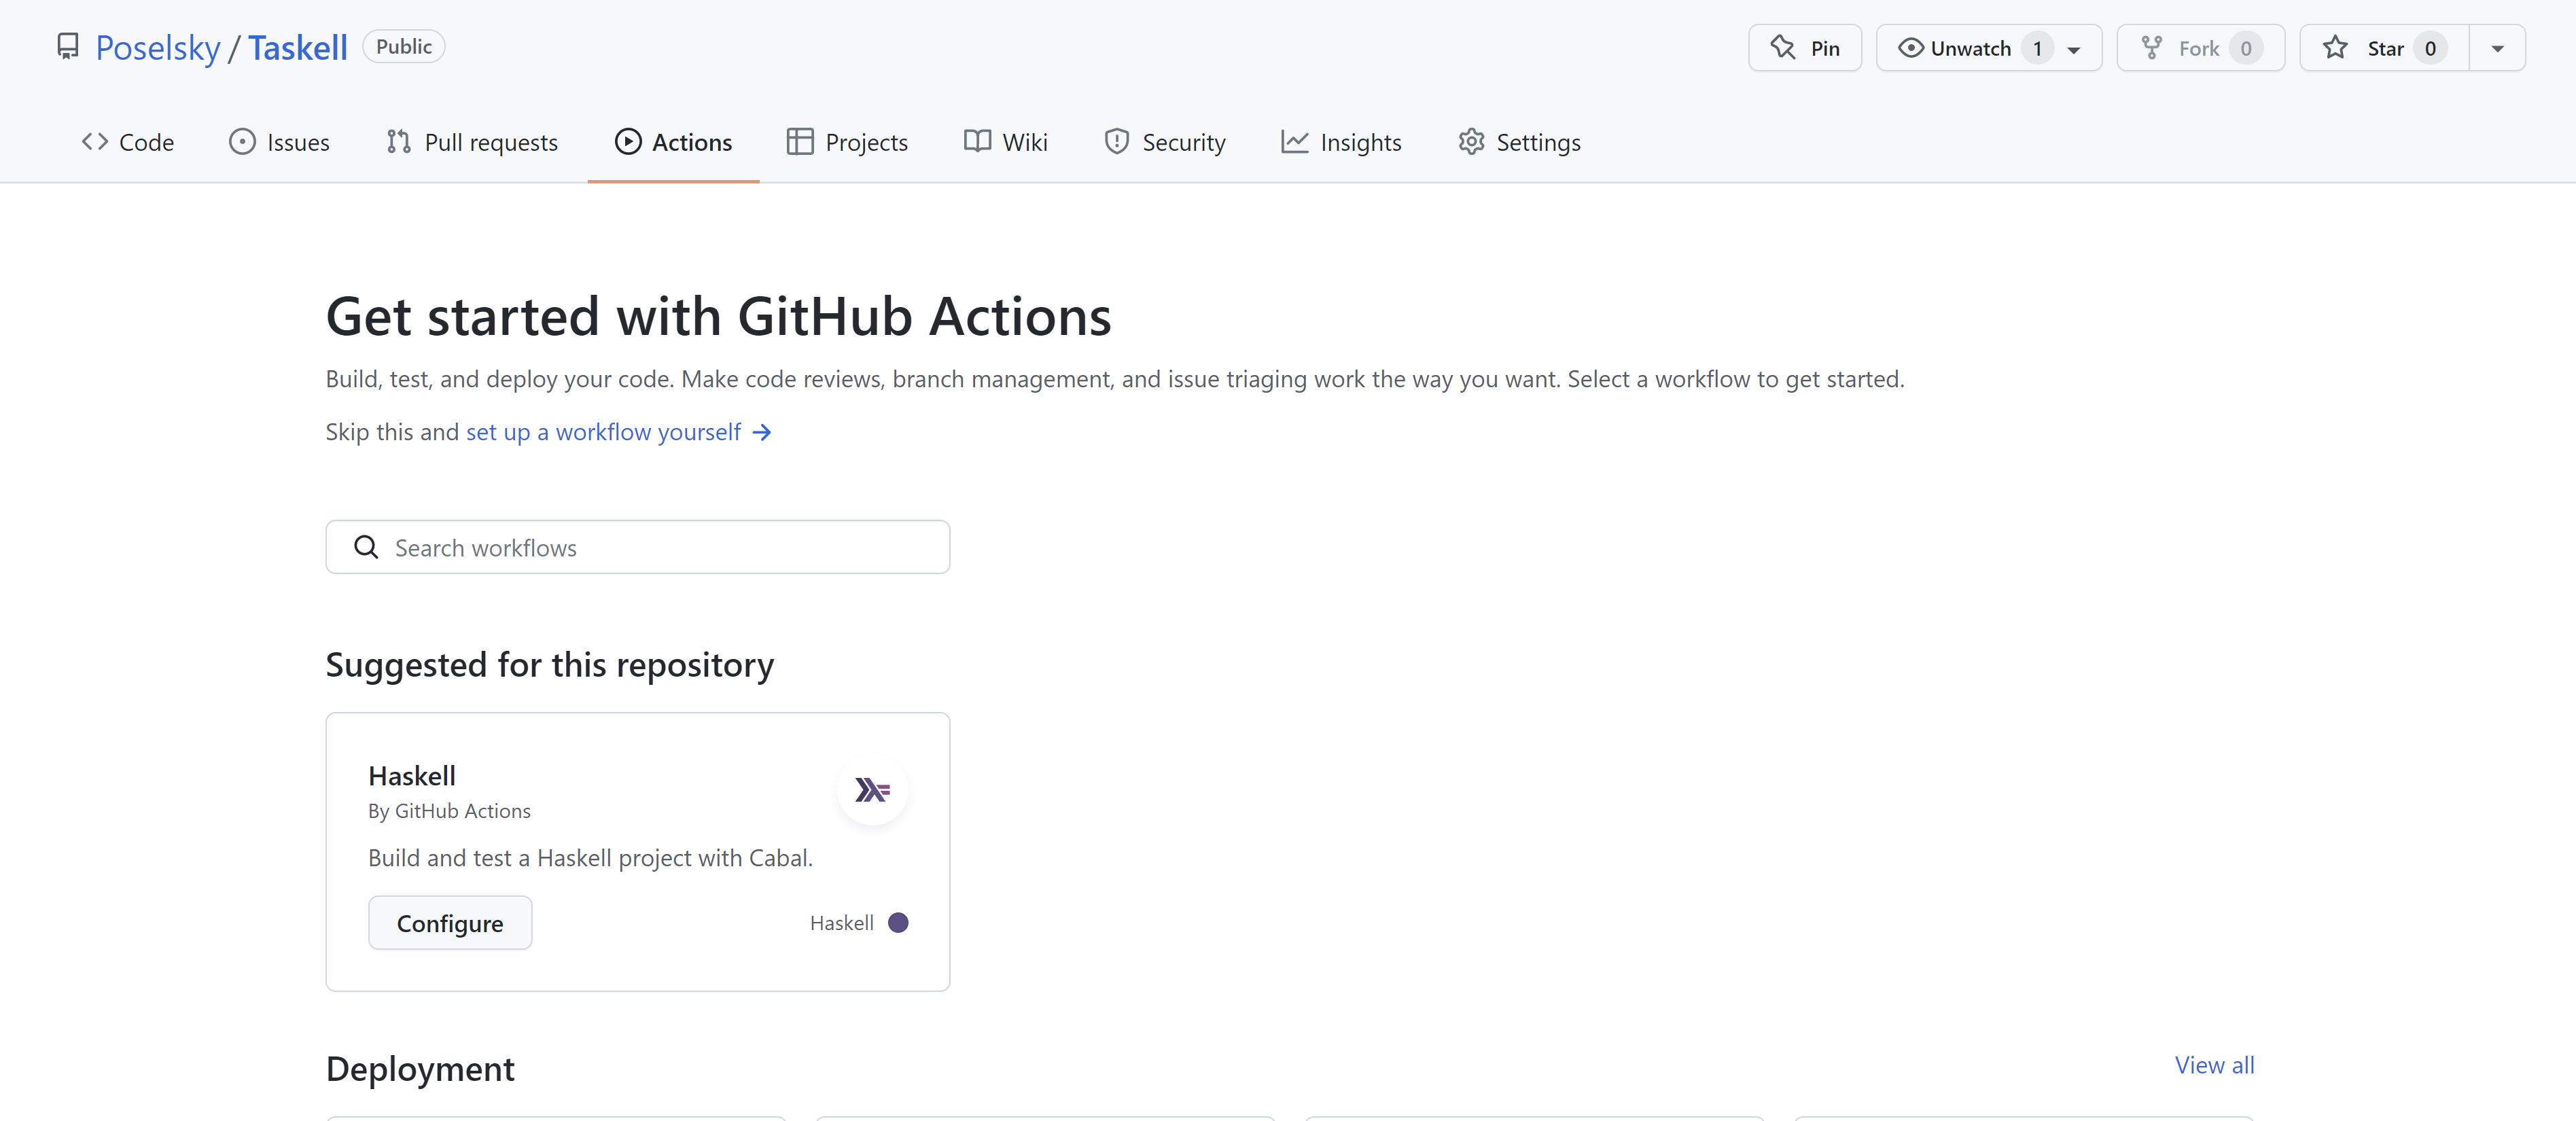
\includegraphics{Deployment.PNG}}
\end{center}
}

\section{Problémy DSL}

Každý projekt si vyžaduje čas, údržbu a dokumentaci.
To se též týká DSL.
Proto je velmi důležité zvážit, 
jestli je užitečné vytvořit DSL nad nějakou knihovnou.
Opravdový problém nastává, 
když je potřeba dané DSL rozšířit nad rámec DSL a
stává se z toho \textbf{Ghetto Language}.
Na tuto problematiku naráží Martin Fowler ve své knize Domain Specific Languages.
Člověk který udržuje dané DSL má za povinost určit meze,
kam bude projekt zasahovat. 
Totiž může nastat situace,
kdy do DSL budou postupně implementovány podmínky,
poté cykly a 
z ničeho nic existuje turingovsky kompletní jazyk, 
který je složitý na pochopení a údržbu. (\cite[s.~38-39]{Fowlerc2011})


\chapter{Návrh vlastního DSL}

Pro návrh DSL je klíčové vědět o jakou doménu problematiky se jedná.
Častým problémem práce s konkurencí je, 
že je mnohdy náročné rozdělit data do jednotlivých transformací bez toho, 
aniž by programátoři vydali obrovské úsilí.
Situace často přerůstá do komplexního problému, 
neboť je nezbytné porozumět, 
kde aplikovat semafory a mutexy. 
V případě výskytu výjimky pak hledání místa, 
kde k výjimce došlo, 
může být vyčerpávající a nervydrásající,
protože vlákna procesoru běží nezávisle na sobě,
tak je tok dat vždy nedeterministický.

Představme si scénář z reálného života, 
na kterém si ukážeme nedeterminismus vláken.
Tři lidé sdílejí domácnost a 
jeden má zaúkol uvařit knedlo vepřo zelo.
Bohužel v lednici se nenacházejí žádné potřebné ingredience,
a tak aby to bylo vůči všem stranám férové,
zbylí dva členové domácnosti musí nakoupit.
V blízkosti se nachází večerka a řeznictví, 
ale bohužel na opačných stranách ulice, 
tak pro urychlení se obě strany dohodnou, 
že se rozdělí na ušetření času.
Zatímco jsou všichni pryč,
kuchař si předpřipravil náčiní a ingredience ze spižírny.
Aby si ušetřil čas, 
tak už dal vodu do kastrolu a nechal si předehřát troubu.
Mezitím se vrátil jeden člen domácnosti s vepřovou krkovicí,
která byla okořeněna a dána do trouby.
Po pár hodinách se vrátil zbývající člen se zbytkem nákupu, 
protože večerka je v neděli zavřená a 
další obchod je pár kilometrů daleko.
Výsledkem celého vaření jsou knedlíky se spálenou krkovicí.

Dalo se tomu předejít,
pokud by se o všechno postaral jeden člen domácnosti.
Ale pokud jsou k dispozici další lidské zdroje pro urychlení práce,
proč je nepoužít?
Samozřejmě toto je celé jen pouze příklad,
jak se může daný program s vícero procesory, 
který má zaúkol uvařit, chovat.
Moderní programovací jazyky programátorům umožňují pracovat s jádry,
ale nedeterministicky a mnohdy s velmi matoucím tokem dat. 

Zatím neexistuje žádná DSL implementace pro konkurenci a
paralelizaci vysokého objemu dat.
Příkladem vysokého počtu dat je vzorek signálu a 
detailnější zpracování takového vzorku je časově velice náročné. 
Tato časová náročnost může být vyřešena právě zmíněnou konkurencí, 
či paralelizací problému. 
Toto DSL je pojmenované jako \textbf{Haskelyzer}.
Pro řešení této problematiky byl zvolen Haskell, 
jelikož se zdá jako nejoptimálnější pro rozbor jazyka,
kde jsou komunitami vytvořené knihovny Parsec, MegaParsec a AttoParsec.
Zároveň Haskell je navržen tak, 
že každá hodnota se chová jako konstanta, 
tudíž nemouhou být pozměněny (kromě pár vyjímek),
což dělá skvělého kandidáta na implementaci paralelních výpočtů.
Obsahuje mechaniky tacit programmingu, 
je staticky silně typovaný a díky monádám, 
řešení okrajových případů jsou donucené GHC kompilátorem.

Hlubokou inspirací sloužila funkcionalita rozšíření "Arrows" 
v jazyce Haskell. % TODO: https://en.wikibooks.org/wiki/Haskell/Understanding_arrows
Toto rozšíření umožňují efektivnější propojení transformací dat.
Ovšem,
i když arrows přináší vylepšený zápis toku dat,
narážíme na problém,
kde samotný tok dat není zcela transparentní.
Navzdory tomu,
že arrows poskytují lepší zápis pro manipulaci s daty,
není jasně oddělen od zbytku Haskell kódu.
V jiných programovacích jazycích,
jako je Python nebo F\#,
existuje také operátor pro předávání dat nazývaný "pipe",
avšak v těchto jazycích slouží pouze k spojování dat bez dalších syntaktických ozdob.
Pozoruhodným rysem těchto šipek je fakt,
že jsou zapisovány tacitně.

\section{Vysvětlení gramatiky jazyka}


\setlength{\parindent}{0pt}
Původní návrh daného jazyka:

\textbf{Haskelyzer}
\begin{minted}[bgcolor=CodeBackGround]{haskell}

[CompileTime]
{
  let exampleCSV = "example.csv" :
    (a,Int)
    (b,Float)
    (c,String)
}

let concurrentProcess = exampleCSV | kalmanFilter 
                                   | gaussianFilter 
                                      

let nestedConcurrentProcess = exampleCSV | kalmanFilter | sum
                                                        | product
                                         | gaussianFilter

\end{minted}

Na uvedém příkladu je vidět,
že jsou zde funkce deklarovány pomocí \haskellInline{let}.
U \haskellInline{exampleCSV} myšlenka byla, 
že při zpracovávání vysokého objemu dat,
tak často dochází k dlouhé prodlevě jen kvůli načtení.
Atribut nad \haskellInline{exampleCSV} 
má 2 možnosti, 
\haskellInline{[RunTime]} a \haskellInline{[CompileTime]}.
V obou případech se
zkontroluje CSV soubor během kompilace, 
zda všechny datové typy souladí s předpisem.
Rozdílem je, 
že v \haskellInline{[CompileTime]} atributu se CSV soubor
stane součástí programu. 
Jednou z nevýhod této metody je, 
že při spuštění programu se zaplní paměť, 
protože obsah csv souboru je součástí samotného spustitelného programu.
Nicméně díky tomu není nutné používat IO monádu a 
obsah csv souboru je k dispozici kdekoliv v programu.
Při procesu kompilace se též provádí kontrola, 
zda v csv souboru existuje dvojice "(a, Int)", 
kde "a" představuje název sloupce a 
všechny hodnoty ve sloupci "a" jsou typu "Int".
To stejné platí pro ostatní dvojice, 
kde sloupec b má být typu Float a tak dále.

Pro vytvoření konkurentního výpočtu je zapotřebí využít \textit{concurrent pipe compostion}
\haskellInline{ | } operátoru. 
Každý další \haskellInline{ | } vytváří dálší vlákno na kterém je prováděný výpočet.
Celá syntaxe je závislá na odsazení, 
tudíž všechny \haskellInline{ | } musí mít stejné odsazení.

Funkce \textit{concurrentProcess} vytvoří funkci typu \haskellInline{IO ([a],[b])} a 
předpokládá, 
že v programu jsou definované a implementované funkce
\haskellInline{kalmanFilter:: CSV -> [a]} a \\
\haskellInline{gaussianFilter:: CSV -> [a]}. 
Výsledné IO monádě se nelze vyhnout, 
jelikož se jedná o konkurentní proces, 
kde vznikají vlákna v jež jsou provedeny výpočty. 

Příklad s funkcí \haskellInline{let nestedConcurrentProcess} ukazuje, 
že \textit{pipe operátory} se dají vnořovat. 
To znamená, 
že funkce sum i product musí mít typ \\
\haskellInline{sum:: (Num a, Num b) => [a] -> b}. 
Výsledná funkce bude vygenerováná jako typ \\
\haskellInline{concurrentProcess:: (Num a, Num b) => IO((a,b), [c])}.

\section{Refactoring původního designu}

Během implementace DSL se zjistilo,
že vložení CSV souborů do kompilovaného programu se nehodí
kvůli náročnosti na paměť a 
zároveň je zde nevýhodou když je potřeba změnit soubor s daty.
Též došlo k zjištění,
že DSL se nemusí pouze využít na analýzu dat,
ale může se použít pro obecné manažování konkurentních procesů.
Takovým příkladem může být GUI aplikace,
kde k vykreslování dochází na jiném vlákně 
než jsou uživatelské interakce.

\textbf{Haskelyzer}
\begin{minted}[bgcolor=CodeBackGround]{haskell}

let guiMainLoop = | gatherMainState -> writeEventQueue -> render
                  | gatherEventQueue -> fireEventsToMainState

\end{minted}

V GUI aplikacích se vždy nachází hlavní cyklus,
který má zaúkol zpracovat uživatelské akce a 
vykreslit stav programu.
\haskellInline{let guiMainLoop} je příkladem,
jak takový hlavní cyklus může vypadat.
Nedílnou součástí GUI aplikací je stav aplikace a
\textit{EventQueue}, kde
se zaznamenávají všechny interakce uživatele a 
program může s těmito interakcemi pracovat.
Jedním z důvodů proč sbírání uživatelských akcí na jiném vlákně je,
že pokud by celý program běžel pouze na jednom procesoru,
tak některé uživatelské akce mohou bránit vykreslování a
tím by docházelo k zasekáváním programu.
Například přehrávání zvuku musí běžet na jiném vlákně,
protože jinak by se program vyrendroval poté,
až by se dokončilo přehrávání zvuku.

\section{Proč Template Haskell místo LLVM}

Prvopočáteční implementace zahrnovala využití knihovny LLVM,
která má za následek převzít AST a 
převést tento jazyk do LLVM \textit{intermediate representation} (IR) (\cite{IntroToLLVM}).
Bohužel LLVM je knihovna primárně pro tvoření generických programovacích jazyků, 
než na tvoření DSL. 
DSL se dá pomocí této knihovny vytvořit, 
ale pro každou vygenerovanou funkci se musí vytvořit binding mezi IR a
jazykem C, 
který je kompilován pomocí CLANG compileru a Haskellem. 
Toto řešení je rozhodně možné, 
ale zvyšuje to komplexitu projektu a 
jednotlivé bindings mohou též být zdrojem nechtěných bugů. 
Proto se sešlo od implementace pomocí LLVM a
místo toho ho nahradil mechanismus metaprograming Template Haskell.

% \begin{minted}{hs}
% [CompileTime]
% {
%   let exampleCSV = "example.csv" :
%     (a,Int)
%     (b,Float)
%     (c,String)
% }
% \end{minted}

\chapter{Implementace interpretu navrženého DSL}

Návrh jakéhokoliv DSL (a nejen DSL, ale i programovacího jazyka celkově) zahrnuje
\textbf{Lexer, Parser a Abstraktní syntaktický strom (AST)}.

\textbf{Lexer} má zaúkol přečíst soubor a 
najít jednotlivé tokeny v daném souboru.
Tyto tokeny mohou obsahovat metadata, 
jako jsou řádek a sloupec, 
kde se token nachází,
jaký token předcházel a jaký následuje atd... 
Tyto tokeny jsou zpracovány \textbf{parserem}, 
který má zaúkol přečíst tokeny a 
hledat mezi nimi dle předem definované gramatiky vztahy a 
zpracovat je do abstraktního syntaktického stromu. 
AST je výsledek parsování a 
obsahuje všechny definice jazyka.

{\begin{center}
\captionof{figure}{Proces zpracování Haskelyzeru}
\resizebox{16.9cm}{!}{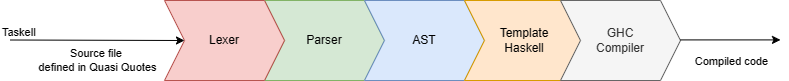
\includegraphics{Parsing.png}}
Zdroj: Vlastní zpracování
\end{center}
}

\section{Parsec a kombinátory}

V tradičních imperativních jazycích parsování probíha pomocí načtení souboru 
do takzvaného \textit{streamu} a 
poté se ze streamu načítají jednotlivé znaky na zpracování tokenů. 
Stream se používá z důvodu konzumace paměti, 
kde každý stream může být naimplementován jinak.
Díky Haskell knihovnám jako je Parsec, 
AttoParsec nebo Megaparsec,
není potřeba zpracovávat jednotlivé znaky, 
ale stačí definovat kombinátory, 
které tyto tokeny vrací. 
Haskelyzer využívá knihovnu Parsec. 
Zde je následující přiklad primitivního kombinátoru.

\begin{minted}[bgcolor=CodeBackGround]{haskell}

import qualified Text.Parsec.Token as Tok
type CustomParser a = Parsec String () a

data Variant = Double | Integer | String deriving Show

emptyLexer:: Tok.GenTokenParser String () Identity
emptyLexer = Tok.makeTokenParser Tok.emptyDef

integer :: CustomParser Variant 
integer = Tok.integer emptyLexer 

float :: CustomParser Variant 
float = Tok.float emptyLexer 

parseToVariant:: CustomParser [Variant]
parseToVariant = many $ integer <|> float <|> 
  (lexeme $ (manyTill alphaNum $ try space))

\end{minted}

Cílem výše zmíněného příkladu je, 
přečíst soubor do \haskellInline{String} 
a rozparsovat ho na list, 
který obsahuje 3 různé datové typy 
a to na \textit{integer, double nebo string}.
Typový synonym \haskellInline{CustomParser a} 
je synonym pro \haskellInline{Parsec String () a},
což znamená, 
že Parsec čte soubor do streamu typu \haskellInline{String}, 
kde nemá žádný stav nebo-li prázdný tuple \haskellInline{()}. 
Parsec je \textit{Monad Transformer},
který zároveň má v sobě zahrnutou stavovou monádu a 
po úspěšném parsování vrací typ a. 

Je nutné zmínit fukci \haskellInline{parseToVariant}. 
Díky kombinačnímu operátoru \haskellInline{<|>} 
lze pouze definovat vysokoúrovňovou parsovací logiku bez potřeby manipulace jednotlivých tokenů. 
Tento operátor funguje na bázi \textbf{alternativa} nebo
\textbf{fallback}. 
Pokud selže parser integer, 
tak se pokusí parsovat float, 
pokud i ten selže, 
tak vždy se rozparsuje poslední možnost a 
tou je jakýkoliv text.

\section{Lexer a hlavní datové typy}

Na začátek je důležité si nadefinovat hlavní datové typy, 
které budou sloužit jako výsledek parsování.
Parsec zprostředkovává jednoduchý token parser, 
který definuje komentáře, 
operátory a rezervovaná jména.
Haskelyzer využívá takzvaný \textit{lexeme} parser.
Tento druh parseru má za úkol ignorovat veškeré whitespace tokeny jako
jsou například tabulátory, 
jednoduché mezery nebo nové řádky.
Díky tomuto druhu parseru se může vývojář pouze soustředit na 
jednotlivé tokeny. 
Naneštěstí knihovna Parsec má v sobě nevyřešené bugy v \textit{lexeme} funkcionalitě, 
které se nemohou opravit, 
protože by se mohly zničit již exisující parsery,
které jsou budovány kolem těchto bugů.
Tento problém není ani správně dokumentován a 
proto se doporučuje místo knihovny Parsec, 
využít v nových parserech knihovnu MegaParsec nebo AttoParsec. 

Definice lexeru si vyžaduje nakonfigurovat jednotlivé parametry,
jako je senzitivita velkých a malých písmen, 
komentáře a rezervovaná jména.

\begin{minted}[bgcolor=CodeBackGround]{haskell}

haskelyzerLexer :: Tok.GenTokenParser String () (IndentT Identity)
haskelyzerLexer =
  Tok.makeTokenParser Tok.emptyDef 
    { 
        Tok.commentStart = "#{",
        Tok.commentEnd = "}#",
        Tok.commentLine = "##",
        Tok.reservedOpNames = ops,
        Tok.reservedNames = names,
        Tok.identStart = letter,
        Tok.identLetter = letter,
        Tok.opStart = oneOf ":!#$%&*+./<=>?@\\^|-~",
        Tok.opLetter = oneOf ":!#$%&*+./<=>?@\\^|-~",
        Tok.nestedComments = True,
        Tok.caseSensitive = True
    }
    where
        ops = ["+","*","-",";", "->" , ":", ",", "|"]
        names = ["let"]

\end{minted}

Lze si všimnout, 
že tato funkce má poněkud zajímavý typ \haskellInline{IndentT Identity}.
Jelikož jazyk nepoužívá středníky a 
místo toho využívá jednotlivá odsazení, 
tak se zde využívá pomocný monad transformer \haskellInline{IndentT} z knihovny \textit{indents}. 
Díky tomu není nutné manuálně počítat jednotlivá odsazení, 
protože budou automaticky započteny v záslosti na zdroji.

Pokud navrhovaný DSL obsahuje nějaké binární či unární operace, 
tak je zapotřebí si definovat do základních stavebních bloků lexeru.

\begin{minted}[bgcolor=CodeBackGround]{haskell}

data BinOp
  = Plus
  | Minus
  | Times
  | Divide
  deriving (Eq, Ord, Show)

data UnaryOp
    = Not
    | Nroot -- Like SquareRoot but N 
    | Exponent
    deriving (Eq, Ord, Show)

type OptionalColumnNameWithType = (Maybe String, CsvDataType)
data Schema = Schema VarNamePath [OptionalColumnNameWithType] 
  deriving (Show, Eq, Ord)

data Expr
  = BinOp BinOp Expr Expr
  | CsvDataType CsvDataType 
  | UnaryOp UnaryOp Expr 
  | Var Name [HaskelyzerFunction]
  | SchemaExpr Schema 
  | LiteralExpr Literal
  deriving (Eq, Ord, Show)

data HaskelyzerFunction = 
  HaskelyzerFunction Name [Name] -- Function name args
  | Concurrent [[HaskelyzerFunction]]
  deriving (Show, Ord, Eq)

data CsvDataType = 
  CsvFloat 
  | CsvInt 
  | CsvString 
  deriving (Show, Ord, Eq)

data Literal = 
  Float Double 
  | Int Integer
  | String String
  deriving (Show, Ord, Eq)

\end{minted}

{
\begin{center}
\captionof{figure}{Lexer v kontextu jazyka}
\resizebox{10cm}{!}{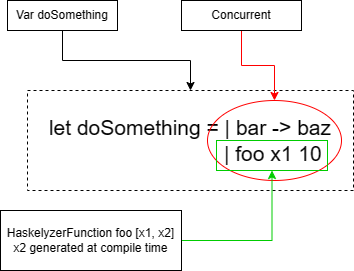
\includegraphics{Taskell-Diagram.png}}
Zdroj: vlastní zpracování
\end{center}
}

\haskellInline{[Expr]} je co tvoří AST.
Seznam jednotlivých \i{expression} je hlavní datový typ všech DSL. 

\haskellInline{Data Literal} jsou pouze primitivní datové typy stejně jako
\haskellInline{CsvDataType}, 
rozdílem je že \haskellInline{CsvDataType} předem definuje, 
zda-li všechny sloupce v CSV souboru jsou očekáváným datovým typem. \\
Typ \haskellInline{OptionalColumnNameWithType} je pro CSV soubory, 
kde CSV soubor má možnost
mít záhlaví a \haskellInline{data Schema} ukládá tuto informaci včetně cestu k tomuto souboru. 

Haskelyzer podporuje vnořené funkce. 
Pro podporu této vlastnosti \haskellInline{HaskelyzerFunction} musí být rekurzivní, 
protože \haskellInline{HaskelyzerFunction} může nabrat formu 
\\
\haskellInline{Concurrent [[Concurrent [[HaskelyzerFunction "Foo" []]]]}
\\
\haskellInline{,[HaskelyzerFunction "Fun" ["arg1"]]]}.

První část \haskellInline{HaskelyzerFunction} je pouze funkce a 
její argumenty, 
druhá část je \\
\haskellInline{Concurrent [[HaskellyzerFunction]]}.
Ve výše zmíněných příkladech bylo poukázáno, 
jak každá vygenerovaná funkce může vytvořit 
další konkurentní funkce a v nich další vnořené konkurentní funkce. 
Díky této vnořenosti 
je potřeba uchovávat funkce v listu listů.

\haskellInline{Var Name [HaskellyzerFunction]} vygeneruje funkci s názvem "Name" a 
pořadí funkcí v \haskellInline{[HaskellyzerFunction]} určují, 
v jakém pořadí budou funkce aplikovány,
v tomto případě jsou \textbf{aplikovány zleva do prava}.

\section{Parser}

Zpočátku se určí tabulka operátorů a 
v jakém pořadí se operátory aplikují, 
poté se tato tabulka předá nultému výrazovému parseru, 
kde tento parser dokáže rozpoznat zda-li výraz patří mezi
hlavní výrazy. 
Zároveň se pro zjednodušení zápisu se definuje typový 
synonym pro parser.

\begin{minted}[bgcolor=CodeBackGround]{haskell}

binary s f assoc = 
  Ex.Infix (reservedOp s >> return (BinOp f)) assoc

table = [[binary "*" Times Ex.AssocLeft,
          binary "/" Divide Ex.AssocLeft]
        ,[binary "+" Plus Ex.AssocLeft,
          binary "-" Minus Ex.AssocLeft]]

type IParser a = 
  IndentParser -- Indent monáda z knihovny indent
    String     -- Vstupní typ, může zde být i Text nebo Bytestring
    ()         -- Stav, v tomto případě stav není zapotřebí
    a          -- Vracející typ po úspěšném parsování

expr :: IParser Expr
expr = Ex.buildExpressionParser table factor

factor :: IParser Expr
factor = 
      try schemaParser 
      <|> try variableParser
      <|> parens factor 

toplevelP :: IParser [Expr]
toplevelP = do 
    def <- many $ do 
        try $ many newline
        s <- expr 
        try $ many newline
        return s
    eof
    return def

parseToplevelP :: String -> Either ParseError [Expr]
parseToplevelP input = 
    runIndent $ runParserT toplevelP () "<stdin>" input

\end{minted}

Funkce \haskellInline{parseToplevelP} je hlavní vstup pro parsování obsahu,
který vrací \textbf{AST}. 
Jelikož typ \haskellInline{[Expr]} je zároveň rekurzivní,
tak tvoří strom - \textbf{AST}.

\section{Testování}

Bez testování parseru by nevznikl žádný spolehlivý parser, 
což dělá testovací fázi jakousi nutností.
S každou přidanou větví parseru musí být přidaná další část v testování,
kterou tuto větev prošetří. 
Logika testování parseru stojí pouze na tom,
že se předá jednoduchý vstup ve formě řetězce nebo souboru
a předpokladá se, 
že výstup parsování bude identické jako předem definované AST.
V testovací fázi se hodí též přidat i vyjímky,
které by měli parsování selhat.

\section{Z AST do Template Haskell}
Template Haskell je rozšíření Haskellu od verze 6, 
který umožňuje typově bezpečné meta-programování během kompilace.
% https://wiki.haskell.org/Template_Haskell
Tím se otevírají možnosti vytvořit funkcionality, 
kde program se může modifikovat sám sebe, 
čemuž se říká \textbf{reflekce}.
Pro tvorbu Haskelyzeru je Template Haskell nedílnou součástí,
bez které se nedá obejít.
Je též možné vytvořit výstupní soubor s vygenerovaným Haskel kódem a 
jej následně umístit do jednotlivých modulů,
ale to nezaručuje, 
že vytvořený program bude typově bezpečný.
Pokud by se chtěla zaručit tato bezpečnost,
tak by se vygenerovaný kód musel projít přes 
Haskell interpreter z knihovny Hint.
Čtenář může usoudit, 
že toto celé je nepotřebně komplexní a 
že je výrazně snažší využít již existujích meta-programming funkcionalit. 

V tuto chvíli jsou zde pouze limitované funkcionality.
Z AST se nyní generují pouze curryované funkce,
kde všechny koncové funkce musí vracet stejný datový typ.

Zde je příklad, 
kde loadModel1 a 
loadModel2 nemusí mít stejný počáteční datový typ, 
ale koncové funkce jako je \haskellInline{scale} 
vrací stejný datový typ \haskellInline{a}.

\textbf{Haskelyzer}
\begin{minted}[bgcolor=CodeBackGround]{haskell}
let loadModels =
| loadModel1 -> rotate 0.0 45.0 90.0 -> scale 4.0
| loadModel2 -> translate 60.0 0.0 0.0 -> scale 3.0
\end{minted}

Při překladu z AST se vygeneruje během kompilace tato funkce.

\textbf{Haskell}
\begin{minted}[bgcolor=CodeBackGround]{haskell}
loadModels:: IO [Model]
loadModels = runListConcurrently [_loadModel1, _loadModel2] 
    where 
      _loadModel1 = 
        ((scale 4.0) . (rotate 0.0 45.0 90.0)) loadModel1
      _loadModel2 = 
        ((scale 3.0) . (rotate 0.0 45.0 90.0)) loadModel2
\end{minted}

Toto je složitější než se na první pohled zdá,
protože celý kontext této funkce se může změnit v ten moment,
kdy se začlení parametry funkce.

\textbf{Haskelyzer}
\begin{minted}[bgcolor=CodeBackGround]{haskell}
let loadModels scaleFactor =
| loadModel1 -> rotate 0.0 45.0 90.0 -> scale scaleFactor 
| loadModel2 -> translate 60.0 0.0 0.0 -> scale scaleFactor 
\end{minted}

\textbf{Haskell}
\begin{minted}[bgcolor=CodeBackGround]{haskell}
loadModels:: Float -> IO [Model]
loadModels scaleFactor = 
    runListConcurrently [_loadModel1, _loadModel2] 
  where 
  _loadModel1 = 
      ((scale scaleFactor) . (rotate 0.0 45.0 90.0)) loadModel1 
  _loadModel2 = 
      ((scale scaleFactor) . (rotate 0.0 45.0 90.0)) loadModel2 
\end{minted}

Prvně se definuje soubor, 
kde se Haskelyzer nachází,
tento soubor se označí jako modul pro kompilátor,
protože veškeré změny v souboru se musí překompilovat. 
Výstup funkce je \haskellInline{[Decl]} obalený 
\haskellInline{Quasi Quotes - Q} monádou.

Nadále se AST zpracuje do jednotlivých, 
kompilátorem podporovaných, 
Haskell funkcí.

\textbf{Haskell}
\begin{minted}[bgcolor=CodeBackGround]{haskell}
generateHaskalyzer:: FilePath -> Q [Dec]
generateHaskalyzer filePath = do
    absoPathTkl <- runIO $ makeAbsolute filePath
    addDependentFile absoPathTkl -- recompile on file change
    -- enable printing during compilation
    runIO $ hSetBuffering stdout NoBuffering 
    runIO $ hSetBuffering stderr NoBuffering 

    ast <- runIO $ readFile filePath >>= parseTopLevelP
    case ast of
      Right exs -> mapM astExprToDec exs
      Left pe -> error $ show pe

astExprToDec:: Expr -> Q Dec
astExprToDec (Var n args haskFunctions ) = do
    let name = mkName n
    liftIO $ print haskFunctions

    -- generate uncapturable names which are not global
    argsAsVarP <- 
        mapM (\x -> do y <- newName x; return (x, y)) args

    let argsMap = Map.fromList argsAsVarP

    haskFunctionsAsExp <- 
        mapM (haskelyzerFunctionToExpr argsMap) haskFunctions
    let result = 
        FunD 
          name 
          [
            Clause 
              (map (VarP . snd) argsAsVarP) 
              (NormalB $ composed haskFunctionsAsExp) 
              []
          ]
    liftIO $ print $ pprint result 
    return result
    where
        composed:: [Exp] -> Exp
        composed (fa:fb:fs) = let composeName = mkName "." in
            foldl 
              (\acc x -> 
                InfixE 
                  (Just x) 
                  (VarE composeName) 
                  (Just acc)) 
              (InfixE (Just fb) (VarE composeName) (Just fa)) 
              fs
        composed [fa] = fa
        composed [] = error "Variable can't be empty"

composeHaskelyzerFunction:: 
  Map String Name -> [HaskelyzerFunction] -> Q Exp
composeHaskelyzerFunction knownArgumentsMap [] = 
  error "Can't compose empty list"
composeHaskelyzerFunction knownArgumentsMap (f:fs) = do
    hf <- haskelyzerFunctionToExpr knownArgumentsMap f
    foldrM helper hf fs

    where
      helper x acc =
        let f = haskelyzerFunctionToExpr knownArgumentsMap x 
          in 
            f >>= \a -> return $ UInfixE a (VarE '($)) acc

haskelyzerFunctionToExpr:: 
  Map String Name -> HaskelyzerFunction -> Q Exp
haskelyzerFunctionToExpr 
  knownArgumentsMap 
  (HaskelyzerFunction name args) = do
    -- Get variables from local parameters, 
    -- if none exist use global ones
    createdArguments <-
            foldrM
                (\arg acc -> 
                  let val = knownArgumentsMap Map.!? arg in 
                  case val of 
                      Nothing -> return (mkName arg:acc) 
                      Just x -> return (x:acc) else 
                ) 
                [] 
                args

    let varsP = map VarP createdArguments 
    let fName = mkName name

    return ( functionApplicationE fName createdArguments)
    -- return (LamE varsP  )

    where
        functionApplicationE:: Name -> [Name] -> Exp
        functionApplicationE functionName (n:ns)= 
          foldr 
            (\x acc -> AppE acc (VarE x) ) 
            (AppE (VarE functionName) (VarE n)) 
            ns
        functionApplicationE functionName [] = 
          VarE functionName

haskelyzerFunctionToExpr knownArgumentsMap (Concurrent fs) = do
    composedFunctions <- 
      mapM (composeHaskelyzerFunction knownArgumentsMap) fs
    AppE (VarE 'runListConcurrently) $ ListE composedFunctions


runListConcurrently:: [IO a] -> IO [a]
runListConcurrently = mapConcurrently id

\end{minted}

\chapter{Praktické příklady využití}

S rozšiřujícím se kódem a funkcionalitou projektu se zvyšuje obtížnost určení, 
kde se nachází problém a jak jsou data distribuována v daném systému. 
Jednou z nejkomplikovanějších výzev při psaní softwaru je jeho škálovatelnost. 
Haskelyzer má výhodu oproti tradičnímu způsobu psaní kódu v tom, 
že nejkritičtější části kódu jsou odděleny od business řešení a nabízejí širší pohled na tok dat. 
To může být z jedním hlavních argumentů, proč toto DSL využí pro větší projekty,
protože usnadnuje jeho škálování.
Vývojáři mají možnost určit, které části jsou nejdůležitější pro daný cíl a zapsat je do Haskelyzeru.

Konkurence má výhodu v tom, že obecně zvyšuje škálovatelnost softwaru, 
ale zároveň přináší složitější stav a zvyšuje riziko výskytu chyb. 
Haskelyzer není pouze DSL pro vnější zápis kritických částí softwaru, 
ale také umožňuje zápis konkurentních výpočtů v snadno čitelné formě. 
Tím vzniká určitá forma samo-dokumentace, 
kterou lze statickým jazykovým analyzátorem převést do UML zápisu.

\section{Využití při načítání 3D modelů a scén}

Skvělým příkladem, kde se dá využit konkurence je při načítání 
scén. Scény jsou tvořeny 3D modely, které mohou být komplexní a 
dlouhé a proto jejich parsování může zabrat hodně času. Pro 
tento příklad byl zvolen vedlejší projekt, který má zaúkol 
vyrenderovat 3D modely pomocí knihovny OpenGL, WaveFront a Lens. 

Knihovna Lens vygeneruje pomocí Template Haskell gettery a settery.
Pomocí těchto vygenerovaných vlastností se dá jednoduším způsobem 
dostat ke vnořeným vlastností dat. 
Třeba operátor (\%\textasciitilde) neboli 'over' přijímá data,
jméno vlastnosti a 
funkci která transformuje pouze danou vlastnost dat.

Vysvětlení samotného rendereru je mimo rozsah této práce, stačí 
pouze vědět, že je zapsán pomocí OpenGL, jelikož tato grafická 
knihovna nemá podporu pro multithreading a renderuje 
3D modely ve Wavefront formátu, 
tak dané modely se musí načíst,
rozparsovat a 
poté vyrenderovat na hlavním vlákně.

\textbf{Haskell}
\begin{minted}[bgcolor=CodeBackGround]{haskell}

data LoadedWaveFrontOBJ = LoadedWaveFrontOBJ {
  -- WaveFrontOBJ from https://github.com/phaazon/wavefront
    _loadedWaveFrontOBJWaveFront:: WaveFrontOBJ
  , _loadedWaveFrontOBJScale    :: GL.GLfloat
  , _loadedWaveFrontOBJTranslate:: Linear.V3 GL.GLfloat
  , _loadedWaveFrontOBJRotation :: Linear.Quaternion GL.GLfloat
} deriving Show

$(makeLenses ''ObjectDescription)

\end{minted}

\textbf{Haskelyzer}
\begin{minted}[bgcolor=CodeBackGround]{haskell}

let loadModels = 
| loadModel1 
| loadModel2 
| loadModel3 
| loadModel4 
| loadModel5 -> rotate 0.0 45.0 90.0
| loadModel6 
| loadModel7 
| loadModel8 
| loadModel9 -> translate 60.0 0.0 0.0 -> scale 3.0
| loadModel10 
| loadModel11 

\end{minted}

Haskelyzer volá funkce na načítání a transformaci modelů.
Je zapotřebí tyto funkce nadefinovat.

\textbf{Haskell}
\begin{minted}[bgcolor=CodeBackGround]{haskell}

$(generateHaskelyzerDSL "pathToHaskelyzer.haskelyzer")

-- define model loading all the way to 11
loadModel1, loadModel2:: IO LoadedWaveFrontOBJ
loadModel1 = parseObj "model1.obj"
loadModel2 = parseObj "model2.obj"

rotate:: 
  GL.GLfloat -> 
  GL.GLfloat -> 
  GL.GLfloat -> 
  LoadedWaveFrontOBJ
rotate degreesX degreesY degreesZ loadedWaveFront = 
  let quat = 
    rotateOnAxis degreesX degreesY degreesZ in 
      loadedWaveFrontOBJRotation %~ ((*) quat) $ loadedWaveFront 

translate:: 
  GL.GLfloat -> 
  GL.GLfloat -> 
  GL.GLfloat -> 
  LoadedWaveFrontOBJ
translate x y z loadedWaveFront = 
  loadedWaveFront & loadedWaveFrontOBJTranslate .~ (V3 x y z)
      
scale:: 
  GL.GLfloat -> 
  LoadedWaveFrontOBJ
scale x loadedWaveFront = 
  loadedWaveFront & loadedWaveFrontOBJScale .~ x

\end{minted}

Funkce \haskellInline{loadModels} vrací typ \haskellInline{IO [IO LoadedWaveFrontOBJ]},
což je pouze vnořená IO monáda, 
která se může usnadnit pomocí pomocné funkce \haskellInline{joinTraversableMonad} a 
to natransformuje data do typu \haskellInline{IO [LoadedWaveFrontObj]}.

\textbf{Haskell}
\begin{minted}[bgcolor=CodeBackGround]{haskell}

joinTraversableMonad:: 
  (Monad m, Traversable t) => 
  m (t (m a)) -> 
  m (t a)
joinTraversableMonad = (sequence =<<)

beforeRendering:: StateT SomeState IO ()
beforeRendering = do
  -- OpenGL and it's shaders are initialized 
  -- and now are ready to receive data on call

  models <- liftIO $ joinTraversableMonad loadModels 

  -- save models to state monad
  modify $ \s -> s & sceneToLoad .~ models

  renderFrame

\end{minted}

Pomocí Haskelyzeru došlo ke splnění cíle.
Konkurentně se načetly modely, 
kde vývojář má kontrolu nad jednolivými vlákny.
Obsah funkce \haskellInline{loadModels} přehledně sděluje cíl,  
případné modifikace jsou uživatelsky přívětivé a 
funkce je zapsaná v tacit formátu.
Modely se načetly před renderováním prvního snímku a 
ty se předají do nějaké stavové monády, 
ze které se poté mohou modely upravovat a renderovat.

Zde je reálná ukázka z rendereru.

\textbf{Haskelyzer}
\begin{minted}[bgcolor=CodeBackGround]{haskell}

let loadModels = 
| loadRook -> scale 10 -> translate 20 0 20
| loadRook -> scale 10 -> rotate (-90) 0 0-> translate 40 0 0
| loadPawn -> scale 10 -> translate 0 0 0
| loadPawn -> scale 20 -> rotate 180 0 0-> translate 100 0 0

\end{minted}

A výsledek po transformacích:

{\begin{center}
\captionof{figure}{Výstřižek z rendereru}
\resizebox{16.9cm}{!}{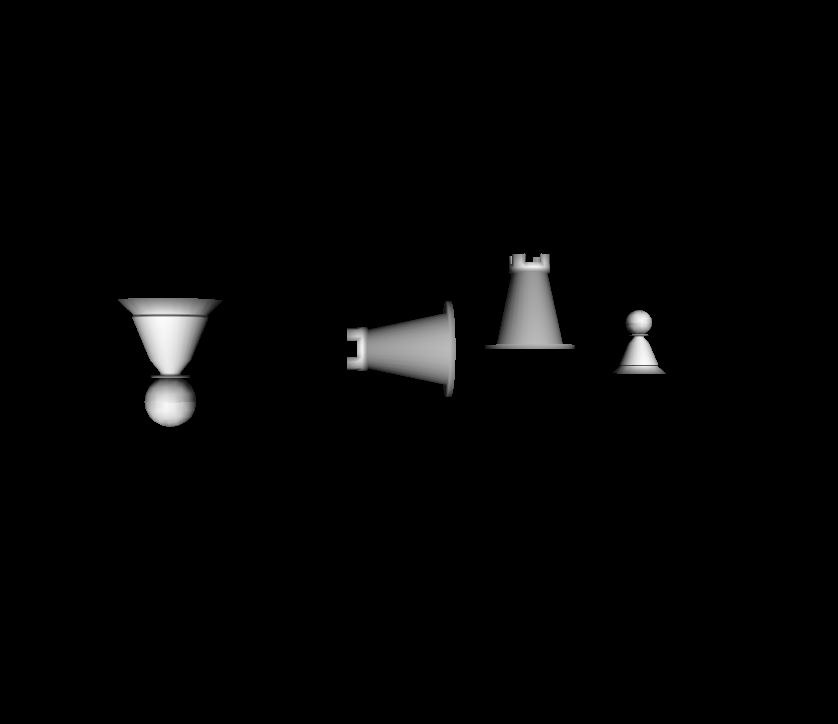
\includegraphics{Renderer-screenshot.png}}
\end{center}
}

\section{Využití pro web scraping}

Haskellyzer zjednodušuje proces web scrapingu. 
Příkladem může být tahání dat z různých veřejných zpravodajských zdrojů a 
následné ukládání výsledků do databáze. 
Spojením s Haskellyzer, knihovnou Scalpel a 
jakýmkoliv databázovým systémem je možné dosáhnout rychlé sbírání dat.

Následující kód předpokládá, 
že jsou vytvořeny tři různé scrapery a 
očekávají url zdroj.
Pro zjednodušení jsou zdroje zapsané ve formě \\ 
\haskellInline{[(String, String, String)]}, 
ale mohou být též v csv formátu.
Cílem je dané výsledky uložit do databáze,
tak je nutné vytvořit konekci k daným databázovým systémům. 

\textbf{Haskell}
\begin{minted}[bgcolor=CodeBackGround]{haskell}

  sourcesFromWhichToMine = 
    [
      ("urlToNewsSource1", 
       "urlToDifferentNewsSource1",
       "urlToWeather1"
      ),
      ("urlToNewsSource2", 
       "urlToDifferentNewsSource2",
       "urlToWeather2"
      ),
      ("urlToNewsSource3", 
       "urlToDifferentNewsSource3",
       "urlToWeather3"
      ),
      ("urlToNewsSource4", 
       "urlToDifferentNewsSource4",
       "urlToWeather4"
      ),
    ]
  
  -- Predefine mining with algorithms here, 
  -- using scalpel is strongly advised
  -- also define saveToPostgreSQL and saveToMongoDB
  createDBConnections:: IO(MongoDBConnection,PostgreConnection)
  createDBConnections = do
    x <- createMongoConnection 
    y <- createPostgreConnection 
    return (x, y)
  
\end{minted}

Dalším krokem je definice způsobu scrapingu. 

\textbf{Haskelyzer}
\begin{minted}[bgcolor=CodeBackGround]{haskell}

let scrapeData a b c postgreConnection mongoConnection = 
  | scrapeNewsSource a -> saveToPostgreSQL postgreConnection
  | scrapeDifferentNewsSource b -> saveToMongoDB mongoConnection
  | scrapeDifferentNewsSource b -> saveToPostgreSQL mongoConnection
  | scrapeWeatherSource c -> saveToPostgreSQL postgreConnection

\end{minted}

Po úspěšném scrapingu se uloží výsledky do specifikované databáze.

\textbf{Haskell}
\begin{minted}[bgcolor=CodeBackGround]{haskell}

scrapeData:: 
  String -> 
  String -> 
  String -> 
  PostgreConnection -> 
  MongoDBConnection -> 
  IO([IO (Bool)]) -- Bool shows if operation was successfull

  -- Predefine mining with algorithms here, 
  -- using scalpel lib is strongly advised
  -- also define saveToPostgreSQL and saveToMongoDB

  $(generateHaskelyzerDSL "pathToFileMentionedAbove")

  beginScraping:: IO ()
  beginScraping = do
    (mongoConnection, postgreConnection) <- createDBConnections
    -- Fire mining, you can potentially wrap this 
    -- into Writer monad to get useful logs
    mapM_ 
      (\(a,b,c) -> 
        scrapeData a b c mongoConnection postgreConnection
      ) 
      sourcesFromWhichToMine <&> sequence . concat
\end{minted}

\section{Využití pro datovou analytiku a změření výkonu}
 
Zpracování dat může zabrat spoustu času, 
jelikož většinou jednotlivé úpravy nad daty běží na jednom vlákně.
Cílem je zjistit zdali clusterování dat pomocí 
Haskelyzeru bude rychlejší než clusterování na jednom vlákně.
Příklad clusteruje 64-dimenzionální data a clusteruje 
od 2 až po 64 clusterů. 
Pro Haskelyzer se rozdělí počet clusterů podle počtu dostupných vláken.

Překvapivě bylo zjištěno, 
že jednovláknová implementace clusterovacího algoritmu 
dosahuje přibližně stonásobně vyšší výkon v porovnání s vícevláknovou variantou. 
Tento výsledek vyvolává otázky o optimálnosti paralelního zpracování v rámci dané úlohy 
a použité implementace.
Jedním z potenciálních důvodů je, 
že vytvoření nového procesu na každém vlákně dodává výkonovou zátěž
a tím se zvyšuje čas pro uskutečnění operace.
Proto je vždy důležité změřit, 
zda-li má smysl přidat pro problém více vláken.

{\begin{center}
\captionof{figure}{Výsledky benchmarkingu, kde je jedno vlákno rychlejší}
\resizebox{16.9cm}{!}{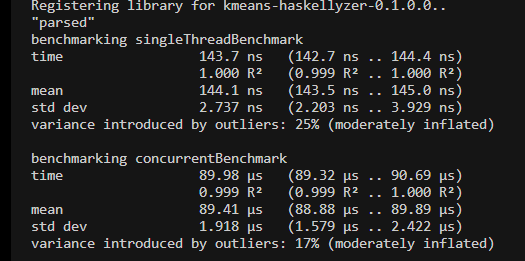
\includegraphics{Benchmark-results-35.png}}
\end{center}
}

\section{Nedostatky a potenciální vylepšení do budoucna}

Do Haskelyzeru byla přidaná funkcionalita na načitání CSV souborů,
kde probíhá validace s možností vkládání dat do programu.
Tato funkcionalita nebyla řádně testována, 
ale nabízí zjednodušení zpracování dat.
Tato funkcionalita se může rozšířit při přidání dalších parserů 
s případnou podporu pro SQL-NOSQL.

Potenciálním vylepšením by bylo ponechaní threadů, 
které by byly znovu využity.
V aplikaci na načítání modelů do scén se nachází pouze část,
kdy se scéna načte pouze jednou.
Ale co se má dít v případě, 
kdy se modely musí načítíst postupně?
Nyní se pokaždé vytvoří nový thread a 
právě tvorba nového threadu zabírá spoustu času,
což bylo možné si povšimnout v třetím příkladu na datovou analytiku.

Nyní Haskelyzer nepodporuje obyčejné konstanty jako argumenty a
spoléhá na konstanty,
které musí místo toho nabízet daný modul, 
kde ja Haskelyzer vyvolán.
Též zde chybí základní podpora foldingu pro sbírání výskedků z Haskelyzeru.

\chapter{Závěr}
Hlavním cílem této práce bylo \textbf{vytvoření doménově specifického jazyka (DSL)} se zaměřením 
na \textbf{tacit (beztečkovou) syntaxi} a 
jak je takový DSL navržen, 
pomocí programovacího jazyka Haskell, 
s ověřením použitelnosti a funkčnosti v různých aplikacích.

V první kapitole je popsáno, 
co vůbec takový tacit zápis je,
v jakém kontextu se dá tacit syntaxe \textbf{využít a naopak kdy se tomu radši vyhnout} a
jak je podporovaný napříč populárními programovacími jazyky,
jako je Haskell nebo Javascript. 
Následně se provádí rešerše nad APL což je programovací jazyk,
který je primárně navržen pro tacit zápis.

V druhé kapitole se nachází \textbf{definice DSL} a
využití různých DSL ve specických doménách problematiky.

V třetí kapitole se nachází \textbf{implementace navrženého DSL}, 
Haskelyzeru, 
který \textbf{řeší problém domény konkurence}.
Jednotlivé sekce obsahují popis navrženého parseru, 
lexeru a 
jak se abstraktní syntaktický strom převádí 
do Haskell kódu během kompilace projektu, 
pomocí \textbf{meta-programming} mechanismu Template Haskell.

V poslední kapitole se \textbf{ověřuje použitelnost} narvženého DSL v 
grafické aplikaci s kontextem načítání modelů do scén,
web scraping aplikaci pro scrapování několika web domén současně a 
datové analýze, 
kde se provádí clustering a zároveň se měří výkon DSL.
Na konci jsou předneseny nedostatky Haskelyzeru a 
potenciální zlepšení do budoucna.

Veškeré přednesené charakteristiky a 
informace o tvorbě DSL v této bakalářské práci
mohou sloužit jako základ pro tvorbu jakéhokoliv DSL v programovacím jazyce Haskell.

\chapter{Citace}


%%\cite{IntroToLLVM}
\printbibliography[heading=none]
\appendix


\chapter{Externí přílohy}

Zdrojový kód DSL se nachází na adrese \href{https://github.com/Poselsky/Haskalyzer}{https://github.com/Poselsky/Haskalyzer}.

Příklad z clusteringu se nachází na odkaze \href{https://github.com/Poselsky/haskell-clustering-example}{https://github.com/Poselsky/haskell-clustering-example}.

\end{document}